\documentclass{beamer}
\usepackage[utf8]{inputenc}

\usepackage{bookman}
\usetheme{Madrid}

% code
\usepackage{xcolor, listings}

\definecolor{dkgreen}{rgb}{0,0.6,0}
\definecolor{gray}{rgb}{0.5,0.5,0.5}
\definecolor{mauve}{rgb}{0.58,0,0.82}

\definecolor{mygreen}{rgb}{0,0.6,0}
\definecolor{mygray}{rgb}{0.5,0.5,0.5}
\definecolor{mymauve}{rgb}{0.58,0,0.82}

\definecolor{f1}{HTML}{AA0000}
\definecolor{f2}{HTML}{00AA00}
\definecolor{f3}{HTML}{AA5500}
\definecolor{f4}{HTML}{0000AA}
\definecolor{f5}{HTML}{AA00AA}
\definecolor{f6}{HTML}{00AAAA}
\definecolor{f7}{HTML}{AAAAAA}

\lstdefinestyle{customc}{
  belowcaptionskip=1\baselineskip,
  breaklines=true,
  postbreak=\mbox{\textcolor{red}{$\hookrightarrow$}\space},
  % morekeywords={*,...},            % if you want to add more keywords to the set
  % deletekeywords={...},            % if you want to delete keywords from the given language
  % escapeinside={\%*}{*)},          % if you want to add LaTeX within your code
  xleftmargin=\parindent,
  language=C++,
  showstringspaces=false,
  % basicstyle=\footnotesize\ttfamily,
  basicstyle={\small\ttfamily},
  keywordstyle=\bfseries\color{green!40!black},
  commentstyle=\itshape\color{purple!40!black},
  identifierstyle=\color{blue},
  stringstyle=\color{orange},
}

\lstset{frame=tb,
  numbers=left,                    % where to put the line-numbers; possible values are (none, left, right)
  stepnumber=1,                    % the step between two line-numbers. If it's 1, each line will be numbered
  % firstnumber=1000,                % start line enumeration with line 1000
  % backgroundcolor=\color{white},   % choose the background color; you must add \usepackage{color} or \usepackage{xcolor}; should come as last argument
  showspaces=false,                % show spaces everywhere adding particular underscores; it overrides 'showstringspaces'
  captionpos=b,                    % sets the caption-position to bottom
  % basicstyle=\footnotesize,        % the size of the fonts that are used for the code
  breakatwhitespace=false,         % sets if automatic breaks should only happen at whitespace
  breaklines=true,                 % sets automatic line breaking
  extendedchars=true,              % lets you use non-ASCII characters; for 8-bits encodings only, does not work with UTF-8
  % frame=single,	                   % adds a frame around the code
  keepspaces=true,                 % keeps spaces in text, useful for keeping indentation of code (possibly needs columns=flexible)
  numbersep=7pt,                   % how far the line-numbers are from the code
  numberstyle=\tiny\color{red}, % the style that is used for the line-numbers
  rulecolor=\color{black},         % if not set, the frame-color may be changed on line-breaks within not-black text (e.g. comments (green here))
  showstringspaces=false,          % underline spaces within strings only
  showtabs=false,                  % show tabs within strings adding particular underscores
  tabsize=2,	                   % sets default tabsize to 2 spaces
  % title=\lstname,                  % show the filename of files included with \lstinputlisting; also try caption instead of title
  % escapechar=@,
  style=customc,
}

% \newcommand{\includecode}[2][c++]{\lstinputlisting[caption=#2, escapechar=, style=custom#1]{#2}<!---->}
% ...

% \includecode{sched.c}
% \includecode[asm]{sched.s}

\newcommand{\code}[1]{\texttt{#1}}
% \newcommand{\code}[1]{\tt{#1}}


\title{Redemption Unit Tests}
\author{Jonathan Poelen}
\institute{Wallix}
\date{17 septembre, 2019}



\begin{document}
\frame{\titlepage}


\begin{frame}
\frametitle{Table of Contents}
\tableofcontents
\end{frame}


\AtBeginSection[]
{
  \begin{frame}
    \frametitle{Table of Contents}
    \tableofcontents[currentsection,currentsubsection]
  \end{frame}
}


\section{Framework de test}

\subsection{Hello World}


\begin{frame}[fragile]
\frametitle{Hello World}

\begin{lstlisting}
#include "test_only/test_framework/redemption_unit_tests.hpp"

AUTO_TEST_CASE(TestRect)
{
    Rect r(10, 110, 10, 10);

    TEST(r.x == 10);
    TEST(r.y == 10);
}
\end{lstlisting}

{\color{f7}tests/utils/test\_rect.cpp(8)}: \textbf{\color{f1}error} in "{\color{f5}TestRect}":
 {\color{f4}check} {\color{f1}r.y} {\color{f3}==} {\color{f1}10 has} failed [{\color{f6}110} {\color{f3}!=} {\color{f6}10}] \newline \newline
\textbf{\color{f1}*** 1 failure is detected in the test module "./tests/utils/test\_rect.cpp"}

\end{frame}


\begin{frame}[fragile]
\frametitle{Objectifs}

\only<1->{Avoir un maximum d'information sur l'erreur}

\begin{itemize}
 \item<2-> Les lignes en cause
 \item<3-> Les conditions d'erreur
 \item<4-> Les valeurs causant une erreur
\end{itemize}

\begin{exampleblock}{}<only@5->
\begin{lstlisting}
bool result = x == 10;
TEST(result); // pas bon
\end{lstlisting}

{\color{f7}tests/utils/test.cpp(42)}: \textbf{\color{f1}error} in "{\color{f5}TestRect}":
 {\color{f4}check} {\color{f1}result} has failed
\end{exampleblock}

\begin{exampleblock}{}<only@6->
\begin{lstlisting}
TEST(x == 10); // bon
\end{lstlisting}

{\color{f7}tests/utils/test.cpp(42)}: \textbf{\color{f1}error} in "{\color{f5}TestRect}":
 {\color{f4}check} {\color{f1}x} {\color{f3}==} {\color{f1}10 has} failed [{\color{f6}110} {\color{f3}!=} {\color{f6}10}]
\end{exampleblock}
\end{frame}


\begin{frame}[fragile]
Un test sans \code{TEST} n'est pas un test !
\end{frame}


\begin{frame}[fragile]
\frametitle{Pas de if}

\begin{itemize}[<+->]
  \item Un bon test limite les \code{if}.
  \item En dehors des boucles, \textbf{0 \code{if}}, car le résultat de la condition \textbf{est} connue à l'avance.
\end{itemize}

\begin{exampleblock}{}<only@3>
\begin{lstlisting}
if (x == 10) { // pas bon
  ....
}
\end{lstlisting}
\end{exampleblock}

\begin{exampleblock}{}<only@4>
\begin{lstlisting}
REQUIRE(x == 10); // bon
....
\end{lstlisting}
\end{exampleblock}
\end{frame}


\subsection{Macro de test}


\begin{frame}[fragile]
\frametitle{Notre framework}
\begin{itemize}[<+->]
 \item Basé sur \textbf{Boost.Test}
 \item Utilise le préfixe \code{RED} plutôt que \code{BOOST}
 \item Ajoute des macros de test spécialisées
\end{itemize}
\end{frame}


\begin{frame}[fragile]
\frametitle{3 niveaux de sévérité}
\begin{itemize}[<+->]
 \item \code{WARN}: simple avertissement
 \item \code{CHECK}/\code{TEST}: incrémente le compteur d'erreur et continue
 \item \code{REQUIRE}: arrêt immédiat
\end{itemize}
\end{frame}


\begin{frame}[fragile]
\frametitle{Macro de comparaison de valeur}
\begin{itemize}[<+->]
 \item \lstinline|TEST(expr)| ou \lstinline|TEST_<level>(expr)|
 \item \lstinline|<level>_CLOSE[_FRACTION](a, b, tolerance)|
 \item \lstinline|<level>_MESSAGE(bool_expr, ostream_expr)}|
 \item \lstinline|<level>_{EQ, NE, LE, LT, GE, GT}(a, b)|
 \item \lstinline|<level>_FILE_CONTENTS(filename, contents)|
\end{itemize}

\begin{exampleblock}{}<only@1>
\begin{lstlisting}
TEST(a == b); // CHECK((a) == (b))
TEST(a < b); // CHECK(a < b)
TEST(a == b +- 2_v); // b - 2 <= a && a <= b + 2
TEST(a < b +- 2_percent); // a < b + b * 2 / 100
\end{lstlisting}
{\color{f7}tests/utils/test.cpp(8)}: \textbf{\color{f1}error} in "{\color{f5}Test}":
 {\color{f4}check} {\color{f1}a} {\color{f3}$<$} {\color{f1}b +- 2\_v has}
 failed [{\color{f6}7} {\color{f3}$>=$} {\color{f6}5+-2 [3, 7]}
\end{exampleblock}

\begin{exampleblock}{}<only@2>
\begin{lstlisting}
// modificateur d'affichage (pour un type compatible avec bytes_view)
TEST(ut::ascii(x), y); // les caractères non ascii sont en héxadécimal
TEST(ut::utf8(x), y); // les caractères non utf8 sont en héxadécimal
TEST(ut::hex(x), y); // tout afficher en héxadécimal
TEST(ut::dump(x), y); // affichage de hexdump
// TEST(ut::ascii(x), y) == TEST(y, ut::ascii(y));
\end{lstlisting}
\end{exampleblock}

\begin{exampleblock}{}<only@3>
\begin{lstlisting}
// seulement pour nombre flottant
CHECK_CLOSE(v1, v2, 0.0001); // 0.0001%
CHECK_CLOSE_FRACTION(v1, v2, 0.0008999);
\end{lstlisting}
\end{exampleblock}

\begin{exampleblock}{}<only@4>
\begin{lstlisting}
CHECK_MESSAGE(a[i], "a[" << i << "] = " << a[i]);
\end{lstlisting}
{\color{f7}tests/utils/test.cpp(8)}: \textbf{\color{f1}error} in "{\color{f5}Test}": {\color{f4}a[1]}
\end{exampleblock}

\begin{exampleblock}{}<only@5>
\begin{lstlisting}
CHECK_EQ(a, b); // CHECK(a == b)
\end{lstlisting}
\end{exampleblock}

\begin{exampleblock}{}<only@6>
\begin{lstlisting}
#include "test_only/get_file_contents.hpp"
CHECK_FILE_CONTENTS("recorder-chunk.pgs",
    R"js({"percentage":100,"eta":0,"videos":1})js");
\end{lstlisting}
{\color{f7}tests/utils/test.cpp(8)}: \textbf{\color{f1}error} in "{\color{f5}Test}":
 {\color{f4}check contents\_\_ == get\_file\_contents(filename\_\_) has failed [100 0 != \{"percentage":100,"eta":0,"videos":1\} ]} \newline
Failure occurred in a following context: \newline
    filename: recorder-chunk.pgs
\end{exampleblock}
\end{frame}


\begin{frame}[fragile]
\frametitle{Error: invalid operands to binary}
\begin{lstlisting}
struct A
{
    bool operator == (A const&) const
    {
        return true;
    }
};

AUTO_TEST_CASE(TestA)
{
    // invalid operands to binary expression
    // ('const A' and 'const A')
    TEST(A{} == A{});
}
\end{lstlisting}
\end{frame}


\begin{frame}[fragile]
Les valeurs doivent pouvoir être affichées, on peut:

\begin{itemize}[<+->]
 \item Tricher
 \item Fournir une surcharge de \lstinline{std::ostream}
 \item Spécialiser une classe \lstinline{TEST_PRINT_TYPE_STRUCT_NAME}
 \item Utiliser \lstinline{TEST_DELEGATE_PRINT}
 \item Ne pas afficher avec \lstinline{TEST_DONT_PRINT_LOG_VALUE(A)}
\end{itemize}

\begin{exampleblock}{}<only@1>
\begin{lstlisting}
TEST((A{} == A{}));
\end{lstlisting}
\end{exampleblock}

\begin{exampleblock}{}<only@2>
\begin{lstlisting}
std::ostream& operator<<(std::ostream& out, A const&)
{
    return out << "A";
}
\end{lstlisting}
\end{exampleblock}

\begin{exampleblock}{}<only@3>
\begin{lstlisting}
template<> struct TEST_PRINT_TYPE_STRUCT_NAME<A>
{
    void operator()(std::ostream& out, A const& /*x*/)
    {
        return out << "A";
    }
};
\end{lstlisting}
\end{exampleblock}

\begin{exampleblock}{}<only@4>
\begin{lstlisting}
TEST_DELEGATE_PRINT(A, "A");

TEST_DELEGATE_PRINT(ns::YYY,
    "YYY{" << int(x) << "}");

TEST_DELEGATE_PRINT_ENUM(ns::YYY);
\end{lstlisting}
\end{exampleblock}
\end{frame}


\begin{frame}[fragile]
\frametitle{Macro de comparaison de séquence}
\begin{itemize}[<+->]
 \item \lstinline|<level>_EQ_COLLECTIONS(first1, last1, first2, last2)|
 \item \lstinline|<level>_EQ_RANGES(rng1, rng2)|
 \item \lstinline|<level>_[SBHC]MEM(bytes1, bytes2)|
\end{itemize}

\begin{exampleblock}{}<only@2>
\begin{lstlisting}
CHECK_EQ_COLLECTIONS(rng1, rng2);
\end{lstlisting}
{\color{f7}tests/utils/test.cpp(8)}: \textbf{\color{f1}error} in "{\color{f5}Test}":
 {\color{f4}check} {\color{f1}::boost::test\_tools::tt\_detail::make\_it\_pair((void("rng1"), begin(a\_\_)), end(a\_\_)) == ::boost::test\_tools::tt\_detail::make\_it\_pair((void("rng2"), begin(b\_\_)), end(b\_\_))} has failed \newline
Mismatch at position 0: 1 != 0.\newline
Mismatch at position 2: 3 != 2.
\end{exampleblock}

\begin{exampleblock}{}<only@3>
\begin{lstlisting}
CHECK_MEM(rng, "viking"_av);
\end{lstlisting}
{\color{f7}tests/utils/test.cpp(8)}: \textbf{\color{f1}error} in "{\color{f5}Test}":
 {\color{f4}check} {\color{f1}rng1\_\_.size()} {\color{f3}==} {\color{f1}rng2\_\_.size() has} failed [{\color{f6}4} {\color{f3}!=} {\color{f6}6}] \newline
Failure occurred in a following context: \newline
    (rng) == ("viking"\_av)\newline
{\color{f7}tests/utils/test.cpp(8)}: \textbf{\color{f1}error} in "{\color{f5}Test}":
 {\color{f4}check} {\color{f1}rng1\_\_} {\color{f3}==} {\color{f1}rng2\_\_ has} failed [{\color{f6}$"\backslash{}x76$}{\color{f1}$\backslash{}x01\backslash{}x02\backslash{}x03"$} {\color{f3}!=} {\color{f6}$"\backslash{}x76"$}{\color{f1}$\backslash{}x69\backslash{}x6b\backslash{}x69\backslash{}x6e\backslash{}x67"$}] \newline
Failure occurred in a following context: \newline
    (rng) == ("viking"\_av)
\end{exampleblock}

\begin{exampleblock}{}<only@4>
\begin{lstlisting}
CHECK_SMEM(rng, "viking"_av);
\end{lstlisting}
{\color{f7}tests/utils/test.cpp(8)}: \textbf{\color{f1}error} in "{\color{f5}Test}":
 {\color{f4}check} {\color{f1}rng1\_\_.size()} {\color{f3}==} {\color{f1}rng2\_\_.size() has} failed [{\color{f6}4} {\color{f3}!=} {\color{f6}6}] \newline
Failure occurred in a following context: \newline
    (rng) == ("viking"\_av)\newline
{\color{f7}tests/utils/test.cpp(8)}: \textbf{\color{f1}error} in "{\color{f5}Test}":
 {\color{f4}check} {\color{f1}rng1\_\_} {\color{f3}==} {\color{f1}rng2\_\_ has} failed [{\color{f6}v}{\color{f1}$\backslash{}x01\backslash{}x02\backslash{}x03"$} {\color{f3}!=} {\color{f6}v}{\color{f1}iking}] \newline
Failure occurred in a following context: \newline
    (rng) == ("viking"\_av)
\end{exampleblock}

\begin{exampleblock}{}<only@5>
\begin{lstlisting}
CHECK_BMEM(rng, "viking"_av); // byte (hexa)
CHECK_HMEM(rng, "viking"_av); // dump format
CHECK_CMEM(rng, "viking"_av); // ascii format
\end{lstlisting}
\end{exampleblock}
\end{frame}


\begin{frame}[fragile]
\frametitle{Macro pour les appels de fonction}
\begin{itemize}[<+->]
 \item \lstinline|<level>_FUNC(function)((args...) @ xxx)|
 \item \lstinline|<level>_FUNC_CTX(function)|
 \item \lstinline|<level>_INVOKER(function)|
\end{itemize}

\begin{exampleblock}{}<only@1>
\begin{lstlisting}
TEST_FUNC(strlen)((str) == len);
\end{lstlisting}
{\color{f7}tests/utils/test.cpp(8)}: \textbf{\color{f1}error} in "{\color{f5}Test}":
 {\color{f4}check} {\color{f1}fctx\_\_8(str)} {\color{f3}==} {\color{f1}len has} failed [{\color{f6}strlen(plop)= 4} {\color{f3}!=} {\color{f6}3}]
\end{exampleblock}

\begin{exampleblock}{}<only@2>
\begin{lstlisting}
// globale ou local
auto fsize = TEST_FUNC_CTX(filesize);
TEST(fsize(filename) == size);
\end{lstlisting}
\end{exampleblock}

\begin{exampleblock}{}<only@3>
\begin{lstlisting}
// local
auto foo = TEST_INVOKER(obj.foo);
TEST(foo(x) == y);
\end{lstlisting}
\end{exampleblock}
\end{frame}


\begin{frame}[fragile]
\frametitle{Vérification d'exception}

\begin{itemize}[<+->]
 \item \lstinline{<level>_NO_THROW(stmt)}
 \item \lstinline{<level>_THROW(stmt, exception)}
 \item \lstinline{<level>_EXCEPTION(stmt, exception, predicate)}
 \item \lstinline{<level>_EXCEPTION_ERROR_ID(stmt, id)}
\end{itemize}

\begin{exampleblock}{}<only@1>
\begin{lstlisting}
CHECK_NO_THROW(something());
\end{lstlisting}
{\color{f7}tests/utils/test.cpp(8)}: \textbf{\color{f1}error} in "{\color{f5}Test}":
 {\color{f4}exception thrown by something()}
\end{exampleblock}

\begin{exampleblock}{}<only@2>
\begin{lstlisting}
CHECK_THROW(something(), std::runtime_error);
\end{lstlisting}
{\color{f7}tests/utils/test.cpp(8)}: \textbf{\color{f1}error} in "{\color{f5}Test}":
 {\color{f4}exception std::runtime\_error is expected}
\end{exampleblock}

\begin{exampleblock}{}<only@3>
\begin{lstlisting}
CHECK_EXCEPTION(something(), std::runtime_error,
    [](auto& e) {
        return e.what() == "Bibidi Bou"; });
\end{lstlisting}
{\color{f7}tests/utils/test.cpp(8)}: \textbf{\color{f1}error} in "{\color{f5}Test}":
 {\color{f4}exception std::runtime\_error is expected}
\end{exampleblock}

\begin{exampleblock}{}<only@4>
\begin{lstlisting}
CHECK_EXCEPTION_ERROR_ID(
    trans.send("message"_av),
    ERR_TRANSPORT_WRITE_FAILED);
\end{lstlisting}
{\color{f7}tests/utils/test.cpp(8)}: \textbf{\color{f1}error} in "{\color{f5}Test}":
 {\color{f4}check} {\color{f1}e\_\_.id} {\color{f3}==} {\color{f1}ERR\_TRANSPORT\_WRITE\_FAILED has} failed [{\color{f6}10} {\color{f3}!=} {\color{f6}1502}]
\end{exampleblock}
\end{frame}


\begin{frame}[fragile]
\frametitle{Autre macros}
\begin{itemize}[<+->]
 \item \lstinline|TEST_CONTEXT(ostream_expr) { ... }|
 \item \lstinline|TEST_CHECKPOINT(ostream_expr)|
 \item \lstinline|TEST_PASSPOINT()|
 \item \lstinline|FAIL(ostream_expr)|
 \item \lstinline|ERROR(ostream_expr)|
 \item \lstinline|ERROR_COUNT|
\end{itemize}

\begin{exampleblock}{}<only@1>
\begin{lstlisting}
for (auto&& s : {"a", "b", "c"})
{
    TEST_CONTEXT(s)
    {
        std::string x = s;
        x += x;
        TEST(size(x) == 2);
        x.pop_back();
        TEST(size(x) == 1);
    }
}
\end{lstlisting}
\end{exampleblock}

\begin{exampleblock}{}<only@6>
\begin{lstlisting}
for (size_t i; i < len && ERROR_COUNT == 0; ++i)
{
    TEST(R[i] == refR[i]);
    TEST(G[i] == refG[i]);
    TEST(B[i] == refB[i]);
}
\end{lstlisting}
\end{exampleblock}
\end{frame}


\begin{frame}[fragile]
\frametitle{Test case}

\begin{itemize}[<+->]
 \item \lstinline|AUTO_TEST_CASE(test_name) { ... }|
 \item \lstinline|DATA_TEST_CASE(test_name, dataset, varname) { ... }|
 \item \lstinline|BIND_DATA_TEST_CASE(test_name, dataset, varnames...) { ... }|
\end{itemize}

\begin{exampleblock}{}<only@1>
\begin{lstlisting}
AUTO_TEST_CASE(TestFoo)
{
    int x = 1;
    TEST(x == 1);
}
\end{lstlisting}
\end{exampleblock}

\begin{exampleblock}{}<only@2>
\begin{lstlisting}
DATA_TEST_CASE(TestBitmap, (std::array{
    FIXTURES_PATH "/color_image.bmp",
    FIXTURES_PATH "/logo-redemption.bmp"
    FIXTURES_PATH "/red_box.png",
    FIXTURES_PATH "/wablogoblue_220x76.png",
    FIXTURES_PATH "/red_box_20x20.png"
}), filename)
{
    TEST(bitmap_from_file(filename).is_valid());
}
\end{lstlisting}
\end{exampleblock}

\begin{exampleblock}{}<only@3>
\begin{lstlisting}
BIND_DATA_TEST_CASE(TestRdpLogonInfo, (std::array{
    std::tuple{3, "3"},
    std::tuple{5, "5"}
}), number, string)
{
    TEST(std::to_string(number) == string);
}
\end{lstlisting}
\end{exampleblock}
\end{frame}


\subsection{Réécriture d'un test}


\begin{frame}[fragile]
\frametitle{test\_remoteFx}
\begin{exampleblock}{}<only@1>
\begin{lstlisting}
struct CustomGdi : public gdi::NullGraphic
{
    void draw(RDPSurfaceContent const &content)
    {
        testPassed = true;
        testResult = fuzzyCompareImage(content.data);
    }

    bool testPassed = false;
    bool testResult = false;
};

decoder.recv(tilesetStream, cmd, gdi);
TEST(gdi.testPassed);
TEST(gdi.testResult);
\end{lstlisting}
\end{exampleblock}

\begin{exampleblock}{}<only@1,6>
{\color{f7}tests/utils/test.cpp(42)}: \textbf{\color{f1}error} in "{\color{f5}TestRemoteFx}":
 {\color{f4}check} {\color{f1}gdi.testResult} has failed
\end{exampleblock}

\begin{exampleblock}{}<only@2>
\begin{lstlisting}
bool fuzzyCompare(uint8_t b1, uint8_t b2)
{
    return (b1 > b2) ? b1 - b2 : b2 - b1;
}

bool fuzzyCompareImage(const uint8_t * img)
{
    for(uint32_t pixel : refImage) {
        if (fuzzyCompare(*img++, (pixel >> 16) & 0xff) > 1)
         || fuzzyCompare(*img++, (pixel >> 8 ) & 0xff) > 1)
         || fuzzyCompare(*img++, (pixel >> 0 ) & 0xff) > 1)
        return false;
    }
  return true;
}
\end{lstlisting}
\end{exampleblock}

\begin{exampleblock}{}<only@3>
\begin{lstlisting}
void checkCompareImage(const uint8_t *img)
{
    for(uint32_t pixel : refImage) {
        RED_TEST(*img++ == ((pixel >> 16) & 0xff) +- 1_v);
        RED_TEST(*img++ == ((pixel >> 8 ) & 0xff) +- 1_v);
        RED_TEST(*img++ == ((pixel >> 0 ) & 0xff) +- 1_v);
        if (RED_ERROR_COUNT > 0) return;
    }
}
\end{lstlisting}
\end{exampleblock}

\begin{exampleblock}{}<only@4>
\begin{lstlisting}
struct CustomGdi : public gdi::NullGraphic
{
    void draw(RDPSurfaceContent const & content)
    {
        testPassed = true;
        checkCompareImage(content.data);
    }

    bool testPassed = false;
};

decoder.recv(tilesetStream, cmd, gdi);
TEST(gdi.testPassed);
\end{lstlisting}
\end{exampleblock}

\begin{exampleblock}{}<only@5-6>
{\color{f7}tests/utils/test.cpp(42)}: \textbf{\color{f1}error} in "{\color{f5}TestRemoteFx}":
 {\color{f4}check} {\color{f1}$R == ((*refImage >> 16) \& 0xFF) +- 1\_v has$} failed [{\color{f6}0xde} {\color{f3}!=} {\color{f6}0x22+-0x1 [0x21, 0x23]}]

{\color{f7}tests/utils/test.cpp(44)}: \textbf{\color{f1}error} in "{\color{f5}TestRemoteFx}":
 {\color{f4}check} {\color{f1}$B == ((*refImage >> 0 ) \& 0xFF) +- 1\_v has$} failed [{\color{f6}0x22} {\color{f3}!=} {\color{f6}0xdf+-0x1 [0xde, 0xe0]}]
\end{exampleblock}

\end{frame}


\section{Génération de fichier dans un test}

\subsection{Ou l'art des échecs aléatoires}


\begin{frame}[fragile]
\frametitle{Les conflits de nom}

\begin{itemize}[<+->]
 \item Plusieurs tests peuvent générer le même fichier: les tests se courcircuitent
 \item La \textbf{compilation matricielle} génère les mêmes fichiers
 \item Plusieurs \textbf{dépôts} génèrent les mêmes fichiers (Jenkins)
\end{itemize}

\begin{exampleblock}{}<only@2>
\begin{lstlisting}
bjam -j7 toolset=gcc-7 toolset=gcc-8 toolset=clang toolset=icc debug san release
\end{lstlisting}
\end{exampleblock}

\end{frame}


\begin{frame}[fragile]
\frametitle{Une maintenance plus complexe}

\begin{itemize}[<+->]
 \item La génération de fichier supplémentaire n'est pas vérifiée
 \item Il y a du code doublon pour supprimer les tests (avant et après le test)
 \item Des fichiers peuvent subsister dans le dépôt suite à des échecs (\lstinline|git status|)
\end{itemize}
\end{frame}


\subsection{Une solution acceptable}


\begin{frame}[fragile]
\frametitle{WorkingDirectory}

\begin{itemize}[<+->]
 \item Un espace de travail isolé par test (\lstinline{$TMPDIR/TestName@WDName@ModuleName@compiler})
 \item Ajout et suppression de fichier au fur et à mesure + test sur chacun
\end{itemize}

\begin{exampleblock}{}<only@3>
\begin{lstlisting}
AUTO_TEST_CASE(TestA)
{
  WorkingDirectory wd{/*name*/};
  TEST(wd.contents("file1") == str);
  TEST(wd.add_file("file2"));
  TEST(wd.add_files({"file2", "file3", "file4"}));
  TEST(wd.remove_file("file_a"));
  TEST(wd.remove_files({"file_b", "file_c"}));
  RED_CHECK_WORKSPACE(wd);
}
\end{lstlisting}
\end{exampleblock}

\begin{exampleblock}{}<only@4>
\begin{lstlisting}
AUTO_TEST_CASE_WD(TestA, wd)
{
  CHECK_FILE_CONTENTS(wd.add_file("file1"), str);
  wd.add_file("file2");
  wd.add_files({"file2", "file3", "file4"});
  // ...
  wd.remove_file("file_a"));
  wd.remove_files({"file_b", "file_c"});
}
\end{lstlisting}
\end{exampleblock}
\end{frame}


\begin{frame}[fragile]
\frametitle{WorkingFile}

\begin{exampleblock}{}
\begin{lstlisting}
AUTO_TEST_CASE(TestA)
{
  WorkingFile wf{name};
  CHECK_FILE_CONTENTS(wf, str);
}
\end{lstlisting}
\end{exampleblock}

\begin{exampleblock}{}
\begin{lstlisting}
AUTO_TEST_CASE_WF(TestA, wf)
{
  CHECK_FILE_CONTENTS(wf, str);
}
\end{lstlisting}
\end{exampleblock}
\end{frame}


\section{Lancement de test avec bjam}


\begin{frame}[fragile]

\begin{itemize}[<+->]
 \item Les tests sont lancés en même temps que la compilation
 \item L'ensemble des tests seuls se compilent avec \lstinline{bjam tests}
 \item Chaque dossier peut être compilé avec son chemin \lstinline{bjam tests/mod/rdp}
 \item Il est possible de compiler un dossier sans ses sous-dossiers \lstinline{bjam tests/mod.norec}
 \item Ou spécifier un test directement \lstinline{bjam tests/core/RDP/test_remotefx} ou  \lstinline{bjam test_remotefx}
 \item Des scripts d'auto-complétion pour \lstinline{zsh} et \lstinline{bash} se trouvent dans \lstinline{tools/bjam/bjam_completion.*}
\end{itemize}

\end{frame}



\section{Variable de compilation}

\begin{frame}[fragile]

Bjam utilise les variables d'environnement ou l'option \lstinline{-s}

\begin{itemize}[<+->]
 \item \lstinline{export BOOST_STACKTRACE=1}
 \item \lstinline{BOOST_STACKTRACE=1 bjam}
 \item \lstinline{bjam -sBOOST_STACKTRACE=1}
\end{itemize}

\end{frame}


\begin{frame}[fragile]

\begin{itemize}[<+->]
 \item \lstinline{BOOST_STACKTRACE=1} affiche la pile d'appel lorsque qu'un type \lstinline{Error} est construit
 \item \lstinline{NO_FFMPEG}, \lstinline{FFMPEG_INC_PATH}, \lstinline{FFMPEG_LIB_PATH}, \lstinline{FFMPEG_LINK_MODE}
 \item toutes les variables liées à l'installation: \lstinline{INSTALLDIR}, \lstinline{PREFIX}, etc
\end{itemize}

\begin{exampleblock}{}<only@4>
\begin{lstlisting}
    sed -E 's/.*\[ setvar ([^ ]+).*\] ;/\1/;t;d' jam/defines.jam
\end{lstlisting}
\end{exampleblock}

\end{frame}


\subsection{Variables utilisées au runtime}

\begin{frame}[fragile]
\begin{itemize}[<+->]
 \item \lstinline{REDEMPTION_LOG_PRINT=1} permet d'activer ou non les logs dans les tests
 \item \lstinline{REDEMPTION_FILTER_ERROR=ERR_TRANSPORT_NO_MORE_DATA,ERR_SEC} supprime la trace de certaines erreurs
\end{itemize}
\end{frame}


\section{Utilitaires dans tools}

\begin{frame}[fragile]

\begin{itemize}[<+->]
 \item \lstinline{tools/rdpproxy_color.awk}
 \item \lstinline{tools/bjam/unit_test_color.awk}
 \item \lstinline{tools/bjam/bjam_filter.awk}
 \item \lstinline{tools/bjam/bjam_autocompletion.*}
 \item \lstinline{tools/c++-analyzer/*}
\end{itemize}

\begin{exampleblock}{}<only@1>
    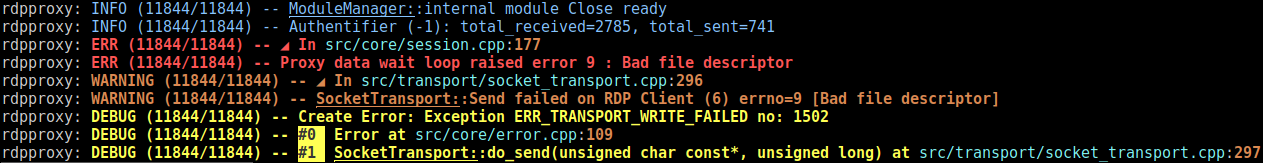
\includegraphics[width=\linewidth]{rdpcolor.png}
\end{exampleblock}

\begin{exampleblock}{}<only@2>
    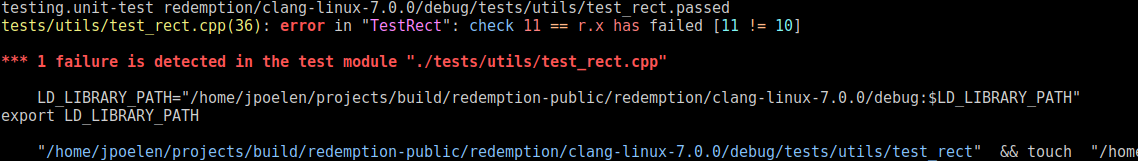
\includegraphics[width=\linewidth]{unittestcolor.png}
\end{exampleblock}

\begin{exampleblock}{}<only@3>
    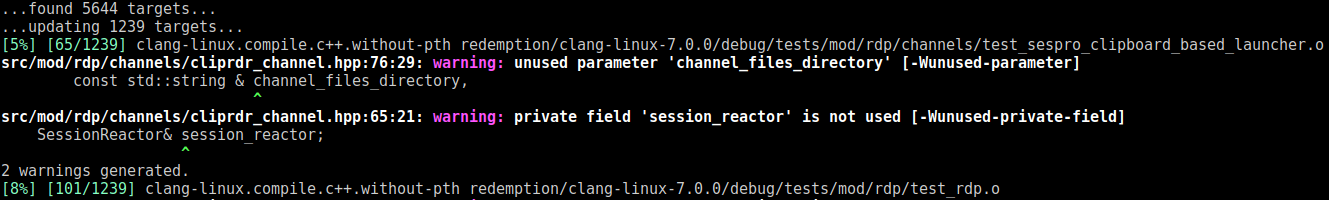
\includegraphics[width=\linewidth]{bjamfilter.png}
\end{exampleblock}

\end{frame}







% \begin{frame}[fragile]
% % \frametitle{Macros de test}
% \end{frame}
% \begin{frame}[fragile]
% % \frametitle{Macros de test}
% \end{frame}

% \begin{frame}[fragile]
% \begin{verbatim}
% your
% code
% example
% \end{verbatim}
%
% aa \code{plop} dsa
% aa \tt{plop} dsa
% \lstinputlisting[breaklines]{source.c}
% \end{frame}

\end{document}

